\documentclass[12pt]{article}

\usepackage{graphicx}
\usepackage{amsmath}
\usepackage{amssymb}
\usepackage{amsfonts}
\usepackage{hyperref}
\usepackage[margin=1in]{geometry}

\title{PHY513 Project Report - Fluid Dynamics Approximation through Machine 
Learning} 
\author{Ximing Qiao}
\date{May 2, 2019}

\begin{document}

\maketitle

\section{Introduction}

Although nonlinear systems are difficult to solve analytically, many practical 
systems exhibits regular patterns. 
Those patterns are difficult to be described analytically, but are still 
evident 
enough for human to recognize. 
People are constantly solving nonlinear systems in their daily lift with 
pattern 
recognition, without even realizing them. 
After some training, students learning nonlinear dynamics can make accurate 
predictions of a system's behavior using very limited information. 
For example, we can project the dynamics to a 2D plane, solve the fixed points 
and their locally linear properties, then fill the non linear part with our 
prior knowledge.

On the other hand, recent advances in machine learning and deep neural networks 
show remarkable results in fitting highly non-linear data, e.g., natural 
images, 
and achieves human-level performance. 
A particularly interesting topic is image-to-image translation.
Given enough training data, a neural network can translate images from an input 
domain to an output domain. 
The neural network uses its learned knowledge to fill the missing information, 
such as texture and color, exactly like how we solve nonlinear systems. 
As such, a natural question rises:
Can we train a machine learning model to predict the behavior of some nonlinear 
systems? 

To utilize the successful experience of applying deep neural networks on 
stationary 2D images, in this project, we focus on studying the steady state 
fluid flow around 2D obstacles.  
We craft a set of training images based on conventional computation fluid 
dynamics method, which numerically simulates the fluid using physical models. 
A deep neural network will fit the data and predict steady state velocity field 
around any unseen obstacle shape.  

From our experiments, we find that a deep neural network can accurately predict 
the fluid dynamics in a limited range. 
This machine learning-based approximation approach cannot be as universal as 
conventional simulation methods, but provide a good speedup when dealing with 
repetitive tasks. 
Examples include boat shape optimization, which requires repetitively 
simulating 
the fluid flow around an obstacle, which change little between each 
optimization 
steps. 
As we can easily parallelize the execution of neural network, the neural 
network-based approximation can achieve over 100$\times$ speedup comparing to 
conventional simulations. 

\section{Background}

\subsection{Computational fluid dynamics (CFD)}

Computational fluid dynamics (CFD) is a type of methods that use numerical 
analysis to solve fluid dynamic problems. 
Usually, a fluid field is described using partial differential equations 
(Navier-Stokes equations, the mass and energy conservation equations, the 
turbulence equations, etc.), and then solved using discrete approximations. 

Solving a steady state fluid dynamic problem with CFD generally follows the 
following steps: 
First, choose an appropriate set of equations according to the problem;
Second, discretize the problem space into many small connected triangles called 
\textit{Mesh}; 
Third, assign boundary condition;
Finally, solve the equations on mesh until the solution converge.
On the other hand, solving turbulence problems might require different 
techniques according the specific problem type to get the best approximation 
results. 

\subsection{Image-to-image translation}

\begin{figure}[htp]
    \centering
    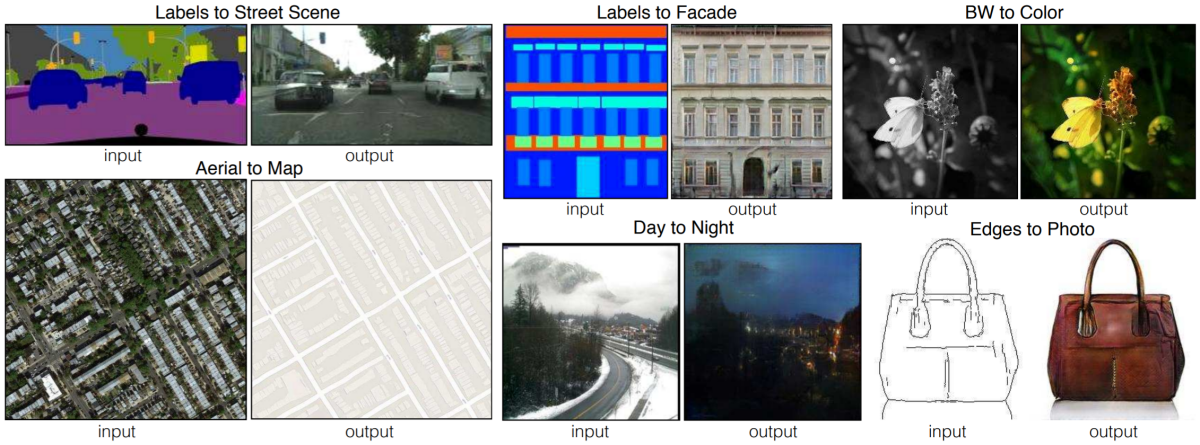
\includegraphics[width=\textwidth]{pix2pix.png}
    \caption{Image-to-image translation examples from~\cite{isola2017image}.}
    \label{fig:pix2pix}
\end{figure}

Recently, generative adversarial nets (GANs)~\cite{goodfellow2014generative} 
was 
introduced as an unsupervised learning method that can generatively model an 
unknown distribution. 
For a probabilistic distribution $f$ with support set $\mathcal{X}$, the 
objective of GAN is to find a generator $G:\mathbb{R}^n\rightarrow \mathcal{X}$ 
such that $G(Z)\sim f$, given $Z\sim \mathcal{N}(0,I_n)$. 
The goal is achieved by assuming a discriminator $D:\mathcal{X}\rightarrow 
{0,1}$ that discriminates a fake sample generated from $G$ against a real 
sample 
obtained from $f$. 
When parameterized as neural networks, both $G$ and $D$ can be trained by 
optimizing the min-max game: 
\begin{equation}
\min_G \max_D \mathbb{E}_{x\sim f}[\log D(x)] + \mathbb{E}_{x\sim G(Z)}[\log 
(1-D(x))]
\end{equation}
through gradient descent.
After convergence, $G(Z)$ should be identical to $f$, and $D$ will output $1/2$ 
everywhere, failing to discriminated fake samples from true samples. 

Conditional GANs~\cite{mirza2014conditional} was later introduced as an 
extension of the original GAN and forms the basis of image-to-image 
translation~\cite{isola2017image}. 
The idea is to extend the loss function in min-max game with a 
\textit{condition}, denoted as $y$: 
\begin{equation}
\min_G \max_D \mathbb{E}_{x\sim f}[\log D(x|y)] + \mathbb{E}_{x\sim 
G(Z|y)}[\log (1-D(x|y))]. 
\end{equation}
The condition can have many possible forms.
When $y$ represent the class label of an image (e.g., cats, dogs, horses, 
etc.), 
the generator is trained to generate images of a particular class. 
When $y$ represents an image, the generator is trained to modify the 
\textit{conditioning image} and match the \textit{target image} from $f$. 

Figure~\ref{fig:pix2pix} shows image-to-image translation examples 
from~\cite{isola2017image}. Conditioning images can be segmentation 
information, black-and-white photos or object edges. Target images can be real 
images with detail texture, colored photos, or object paints. Notice that there 
is no magic in this image-to-image translation.
All the missing information in translation are filled by a neural network 
trained a dataset containing thousands of image \textit{pairs}. 
The neural net learns by analyzing the difference between each pair of images.
Each type of translation is trained on a separate neural network and a 
separated 
dataset, and each neural network works like a ``domain expert'' that can only 
translate one type of images. 



\section{Implementation}

Implementing the machine learning-based CFD approximation includes multiple 
steps, each requires a different software. 

For shape generation, Mathematica~\cite{mathematica} excels at its expressive 
programming language and powerful visualization. 

Mesh generation requires an open-source software Gmsh~\cite{Gmsh}. Gmsh 
supports manual mesh creation though its GUI, but it is too slow to create 
thousands of meshes. Alternatively, we can write a Python script to automate the 
process using Gmsh's Python API. 

After obtaining meshes, we can use a Matlab CFD toolbox 
QuickerSim~\cite{quickersim} for CFD simulation, and continue to use Matlab for 
some image processing to generate training images. 

At last, we use a PyTorch implementation of image-to-image 
translation~\cite{pix2pix} to train and test the neural network. 
The details of each step are described as follows. 

\subsection{Obstacle shape generation}

\begin{figure}[!p]
    \centering
    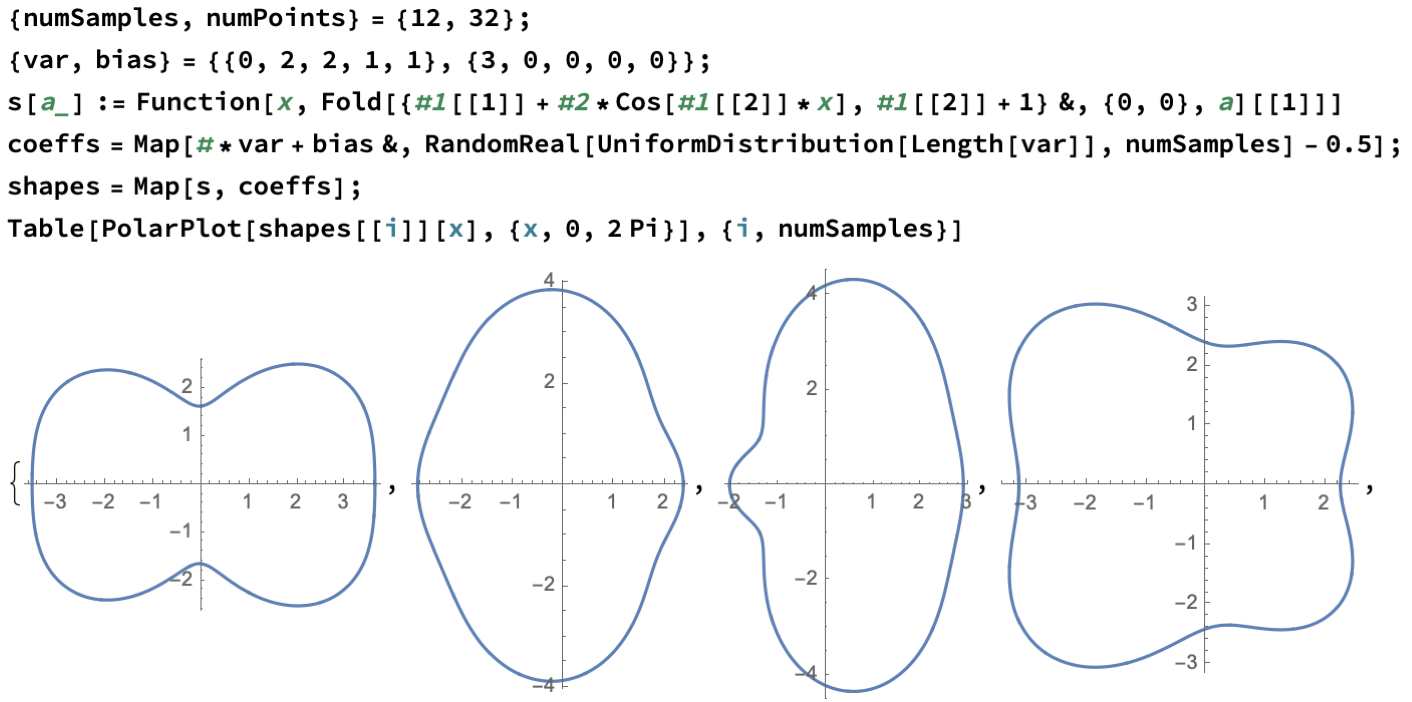
\includegraphics[width=0.75\textwidth]{shapes.png}
    \caption{Mathematica code for simple shape generation.}
    \label{fig:simple-shape}
\end{figure}

\begin{figure}[!p]
    \centering
    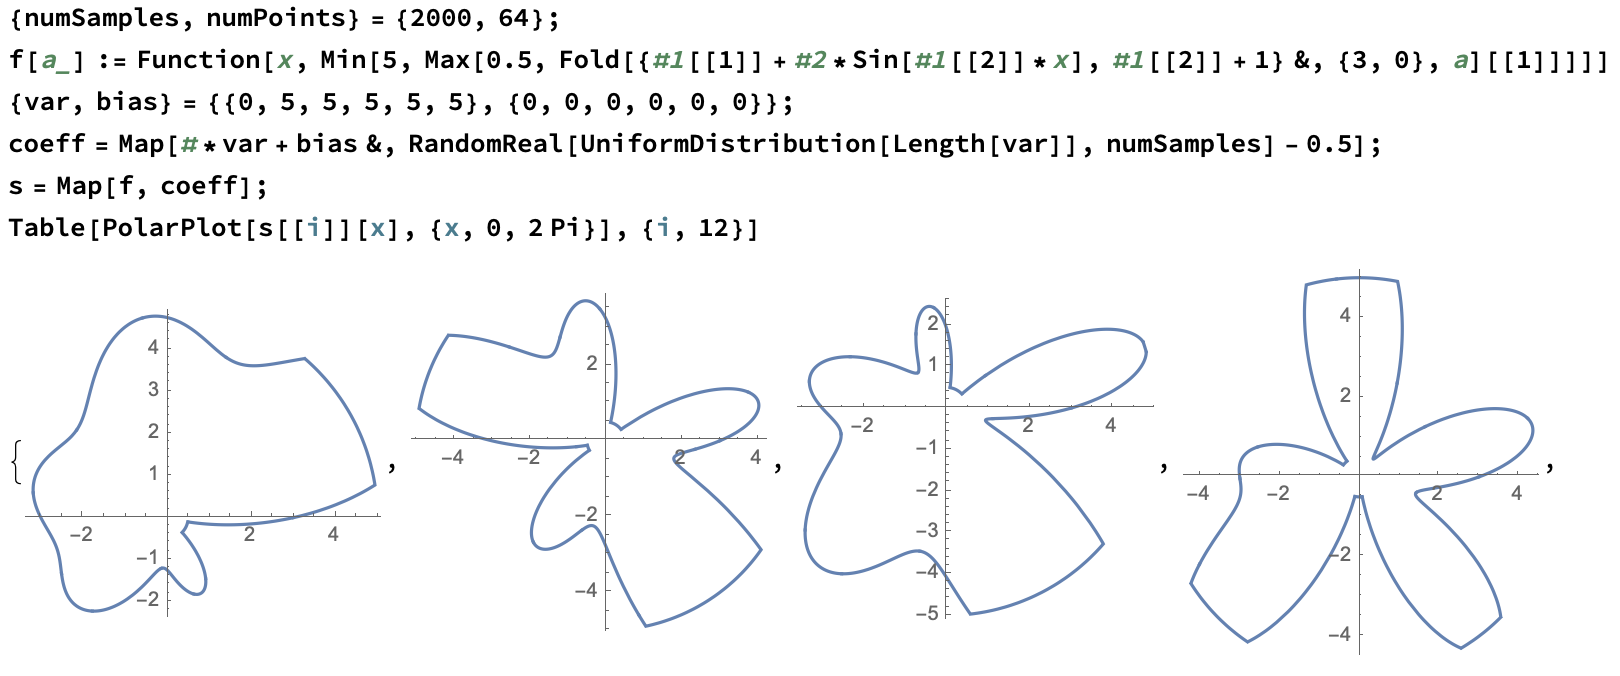
\includegraphics[width=0.85\textwidth]{complex-shapes.png}
    \caption{Mathematica code for complex shape generation.}
    \label{fig:complex-shape}
\end{figure}

\begin{figure}[!p]
    \centering
    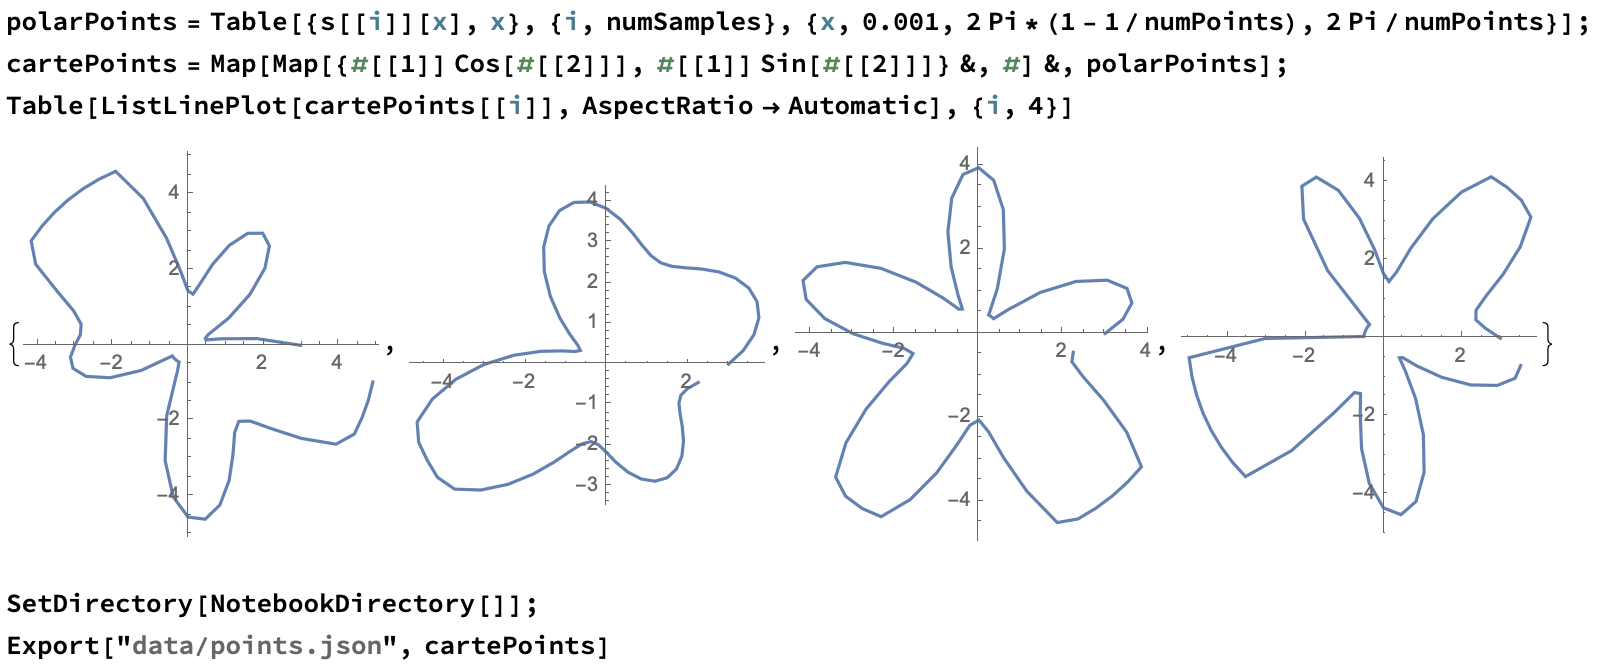
\includegraphics[width=0.85\textwidth]{discretize.png}
    \caption{Discretize the generated shapes and export to a file.}
    \label{fig:discretize}
\end{figure}

We divide the shape generation to two cases: simple shapes and complex shapes.
Simple shapes are generated in polar coordinates, using a linear combination of 
several cosine functions. 
Here we choose 4 fixed frequencies $\omega=1$, $2$, $3$, and $4$.
The amplitudes are sampled from uniform distributions $\mathcal{U}(-1,1)$, 
$\mathcal{U}(-1,1)$, $\mathcal{U}(-0.5,0.5)$, and $\mathcal{U}(-0.5,0.5)$. 
A code snippet of simple shape generation is shown in 
Figure~\ref{fig:simple-shape}. 
Those simple shapes are smooth, symmetric, and similar in size.

The complex shapes are still generated in polar coordinates, but using a linear 
combination of several sine functions, breaking the symmetricy. 
The complex shapes have 5 different frequencies and larger range of random 
amplitudes. 
Several shape examples are shown in Figure~\ref{fig:complex-shape}.
Notice how they differ from the simple shapes.

To turn the generated shapes into meshes, we discretize the curves and turn the 
anchor points into Cartesian coordinates. All the points are exported to a JSON 
file for next step of processing. The code snippet for discretization and 
exporting is shown in Figure~\ref{fig:discretize}.

\subsection{Mesh generation}

\begin{figure}[htp]
 \centering
 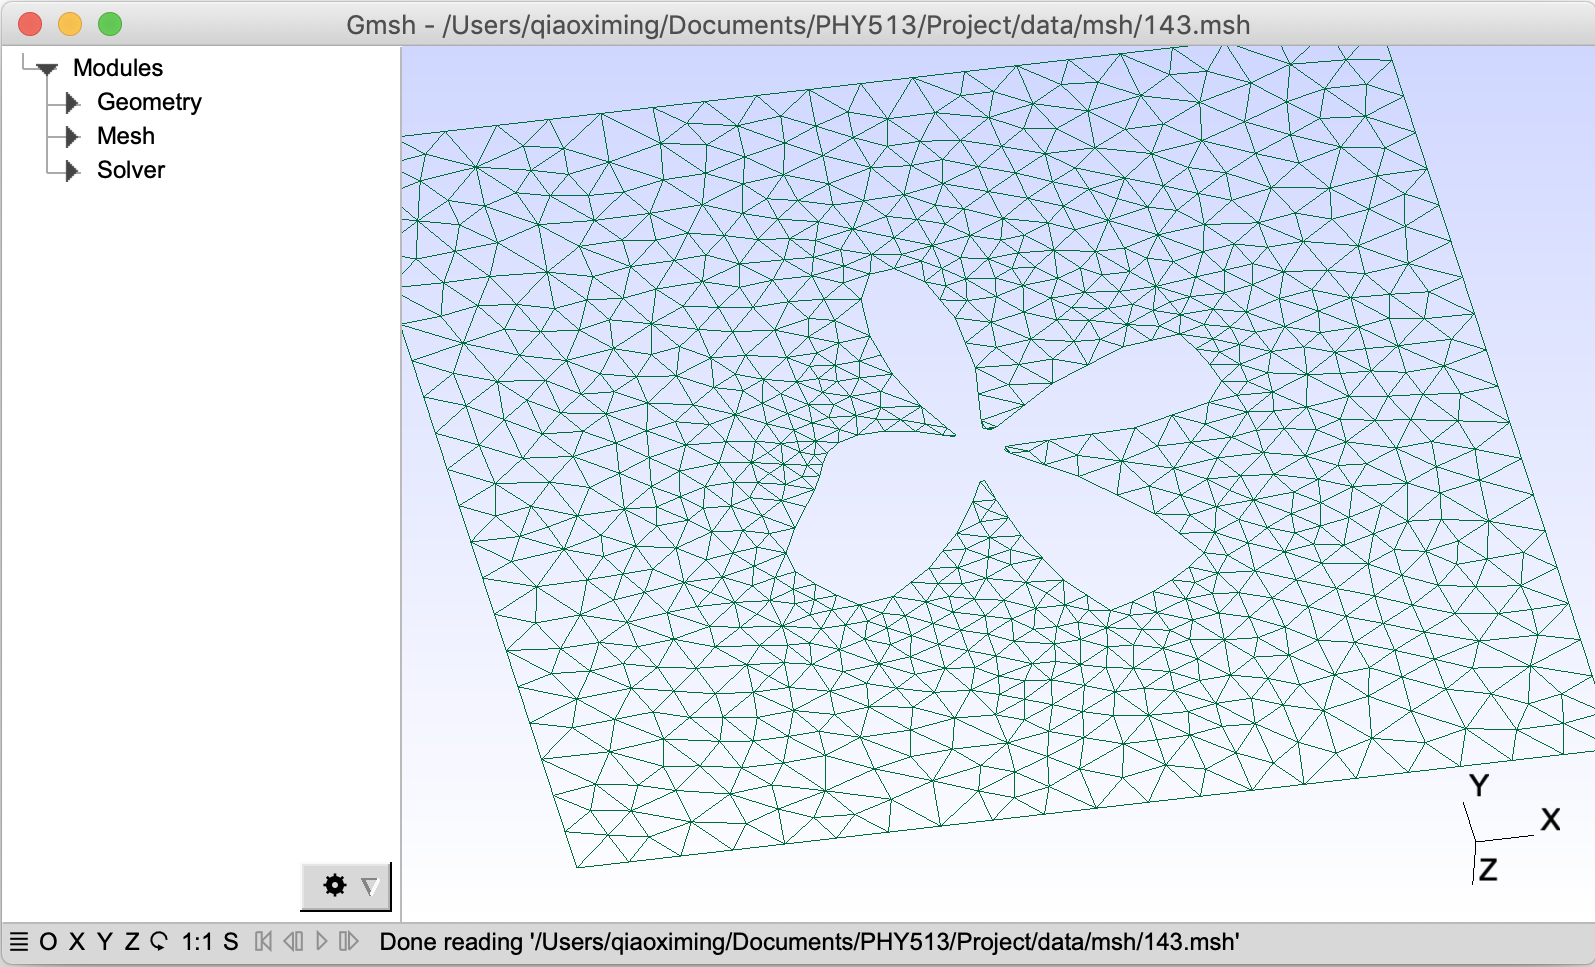
\includegraphics[width=0.7\textwidth]{gmsh.png}
 \caption{Mesh generation using Gmsh's GUI.}
 \label{fig:gmsh}
\end{figure}

\begin{figure}[htp]
 \centering
 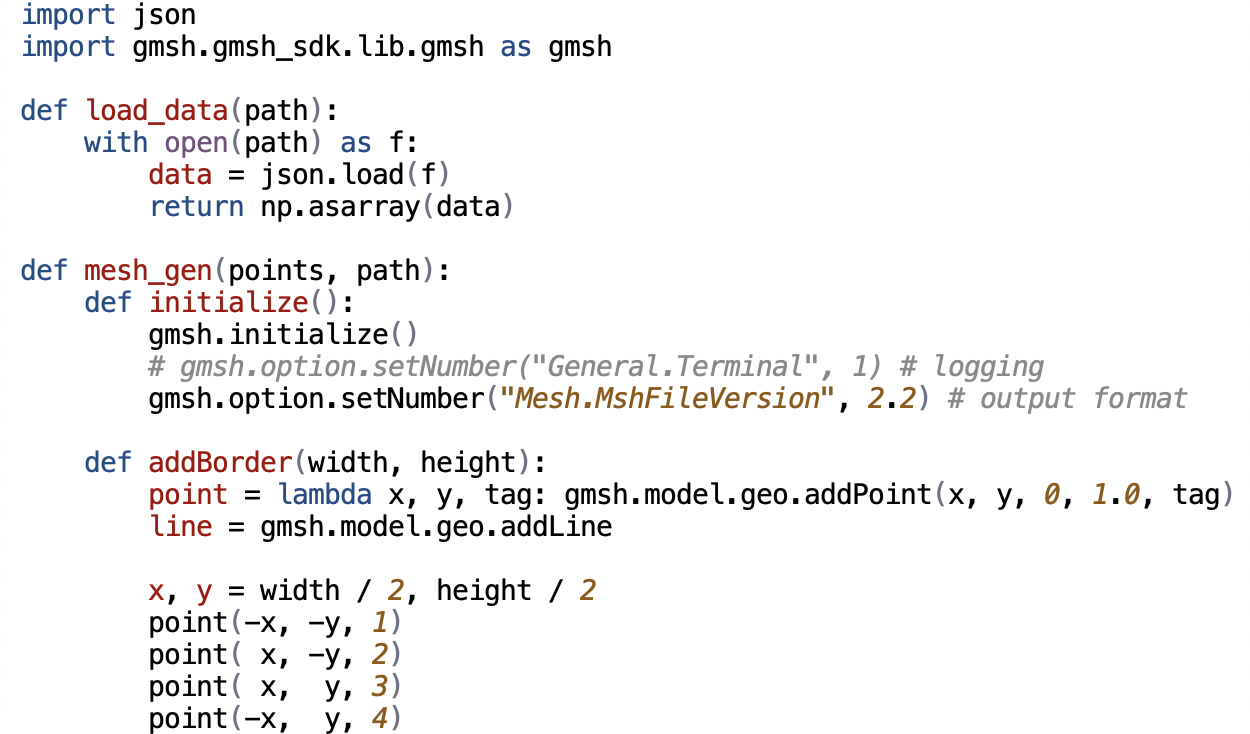
\includegraphics[width=0.6\textwidth]{gmsh-auto.png}
 \caption{Mesh generation using Gmsh's Python API.}
 \label{fig:gmsh-script}
\end{figure}

Gmsh is an open source software for mesh generation. One can use its GUI to 
manually input each anchor points, connect them by lines, and then generate the 
mesh, as shown in Figure~\ref{fig:gmsh}. Obvious, the method is not useful when 
we need thousands of training data to train the machine learning model. 
Instead, Gmsh provides APIs for C++, Python, and other languages to automate 
the process. Here we use Python to convert the anchor points generated in 
previous step to mesh files. A code snippet is shown in 
Figure~\ref{fig:gmsh-script} to demonstrate the process. This step produces 
2000 mesh files for simple shapes and 2000 mesh files for complex shapes.

\subsection{CFD simulation}

\begin{figure}[htp]
 \centering
 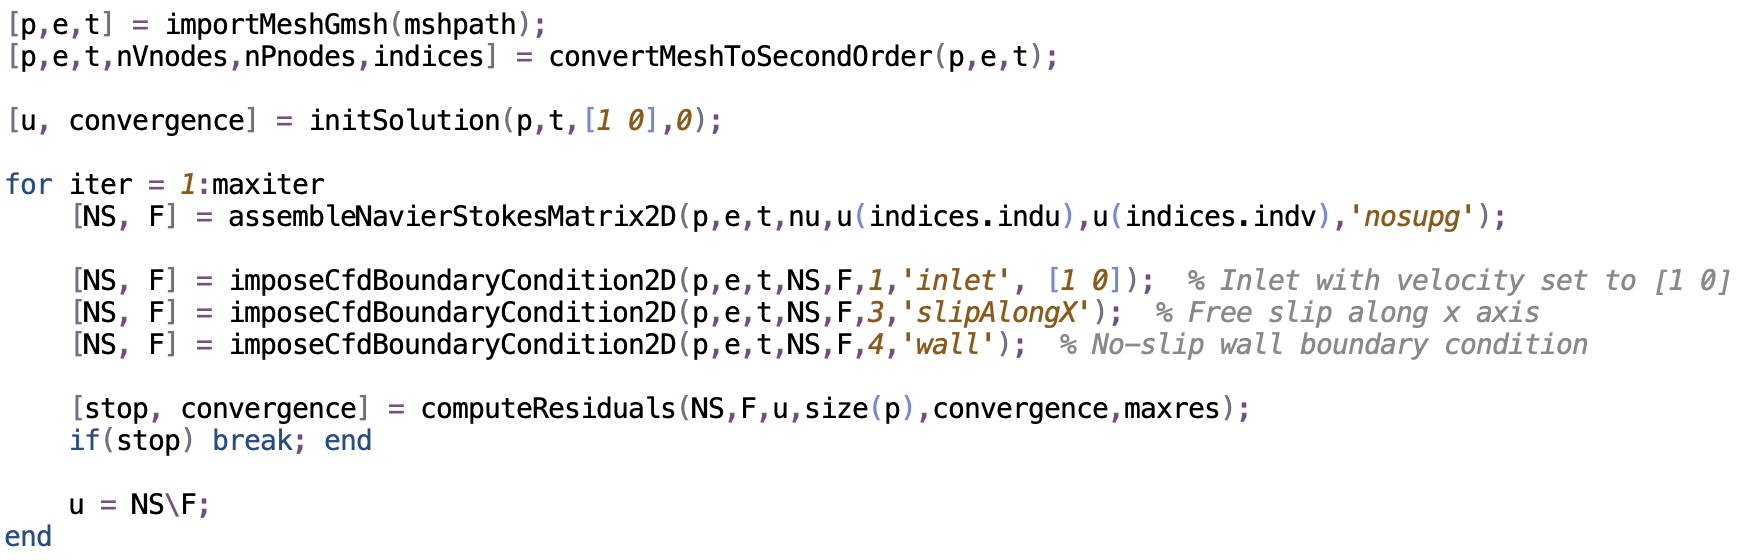
\includegraphics[width=0.9\textwidth]{CFD.png}
 \caption{CFD simulation.}
 \label{fig:CFD}
\end{figure}

\begin{figure}[htp]
 \centering
 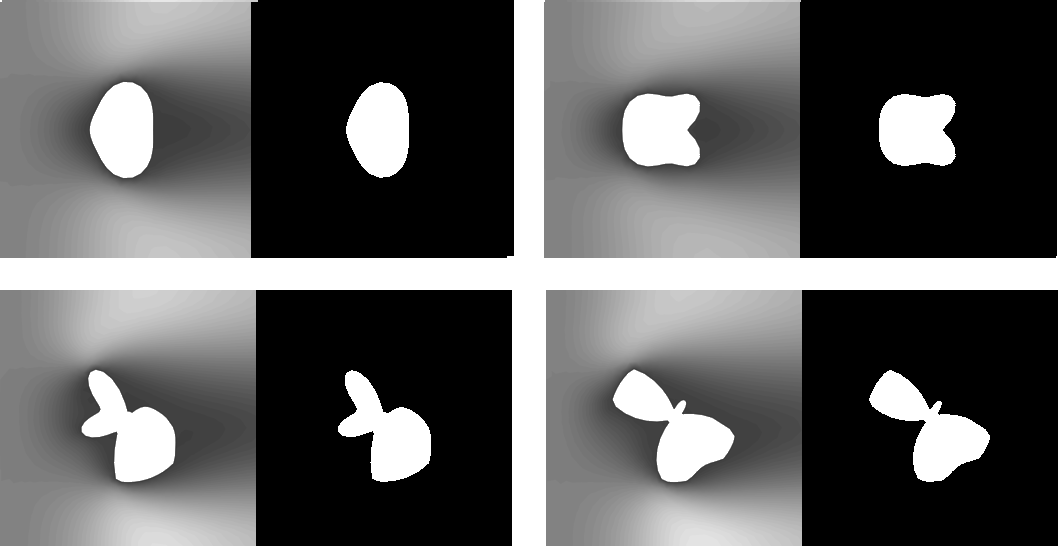
\includegraphics[width=0.8\textwidth]{training.png}
 \caption{Sample training data: velocity field on the left and obstacle shape 
on the right.}
 \label{fig:data}
\end{figure}

The CFD simulation is done in Matlab using a toolbox 
QuickerSim~\cite{quickersim}.
In the simulation, we assign the initial velocity on the left border to be 
$1m/s$ toward right, the friction on upper and lower border to be zero, and the 
right border to be empty.
The toolbox repeatedly solves NS equations until the solution converges.
At last, the obstacle shape and resulted velocity field are exported as 
256$\times$256 images.
Paired images are connected together to form the dataset for neural network 
training.

Figure~\ref{fig:CFD} shows the core of CFD simulation.
Figure~\ref{fig:data} shows some sample image pairs in the dataset.
The right part of each image pair is used as the conditioning image, containing less information (binary color).
The left part of each image pair is used as the target image, containing more information (real-valued color) for the machine learning model to learn.
Each training sample requires about 2 seconds of CPU time to compute. 
The whole process is done within about 3 hours. 

\subsection{Neural network training}

Given the paired images generated from previous step, we split them by 
90\%/10\% for training and testing.
We use a PyTorch implementation of image-to-image translation~\cite{pix2pix} 
with has good support of GPU acceleration.
For each case (simple shapes or complex shapes), we train a separate neural 
network on 1800 images pairs for 50 epochs, and then use the other 200 images 
for testing.

\section{Results}

\subsection{Simple shapes}

\begin{figure}[p]
 \centering
 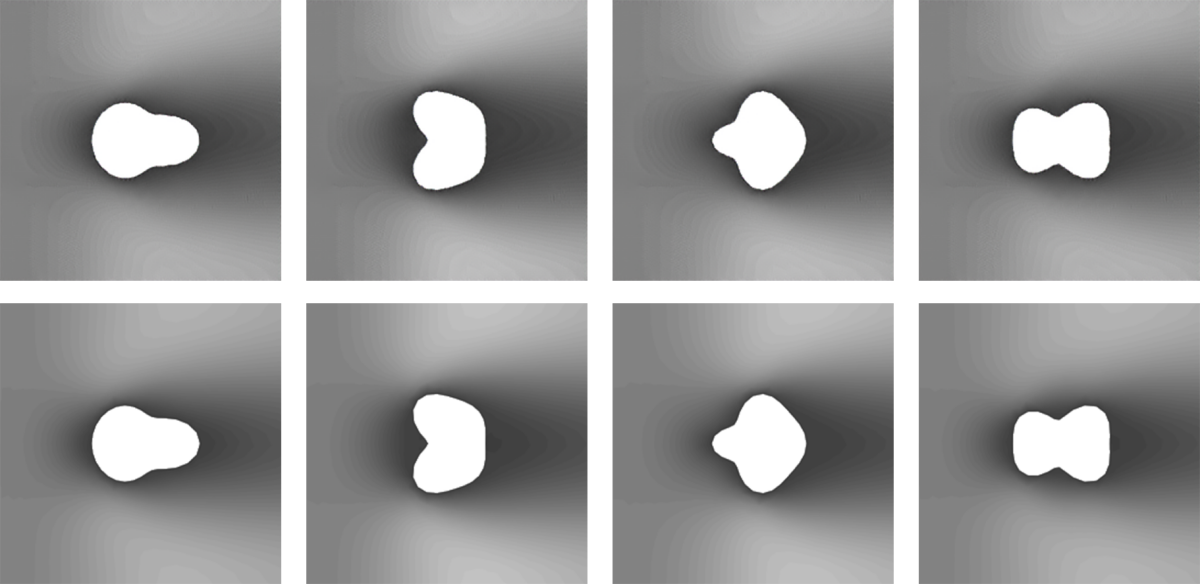
\includegraphics[width=\textwidth]{result.png}
 \caption{Results on simple shapes. The upper row is neural network's 
prediction. The lower row is the simulated ground truth.}
 \label{fig:result1}
\end{figure}

\begin{figure}[p]
 \centering
 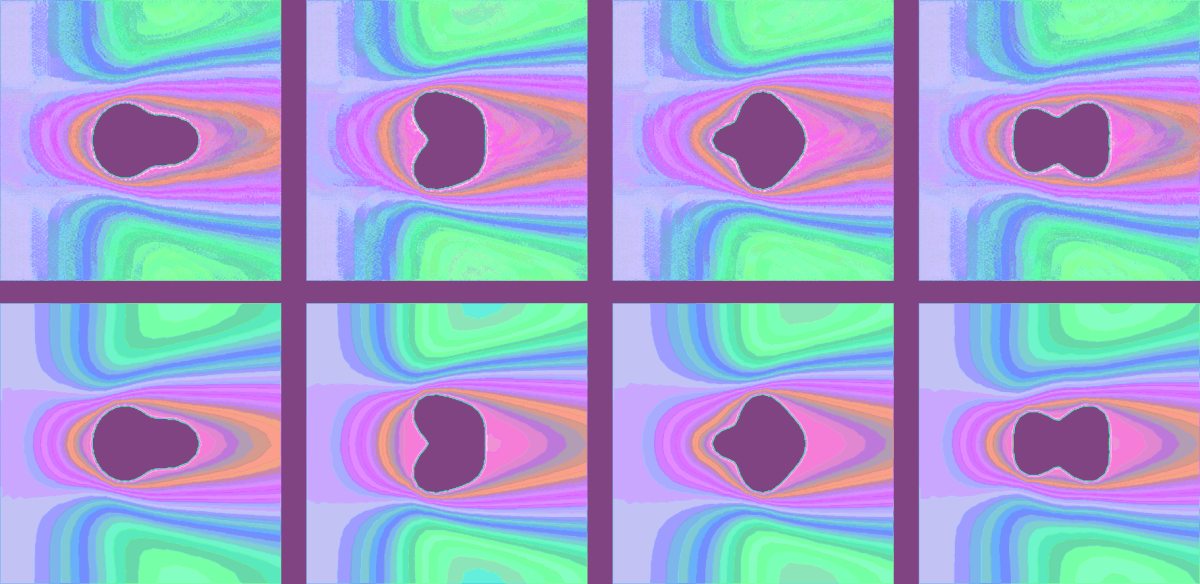
\includegraphics[width=\textwidth]{result-color.png}
 \caption{Results on simple shapes. Each gray-scale color is randomly replace 
by another color for better visualization.}
 \label{fig:result1c}
\end{figure}

We first show the results on simple shapes. Figure~\ref{fig:result1} shows some randomly picked prediction results on the upper row, and corresponding ground truth images on the lower row. 
The neural network can correctly identify the obstacles' shapes and color the surroundings dark. 
The dark ``band'' on the right hand side of obstacles are also correctly color, which have their height depending on the height of obstacles.
The bright ``wings'' on top and bottom of the images are correctly predicted, with their brightest color (highest velocity) decided by the height of obstacles.
The neural network can correctly learn to use global information and predict long-range dependencies.

Figure~\ref{fig:result1c} is a recolored version of Figure~\ref{fig:result1}, better visulizing the details.
We can observed that the neural network can learn the symmetric shape of contour lines, but introduce extra noise.
The prediction results could be further improved by some basic post-processing such as smoothing.

\subsection{Complex shapes}
\begin{figure}[p]
 \centering
 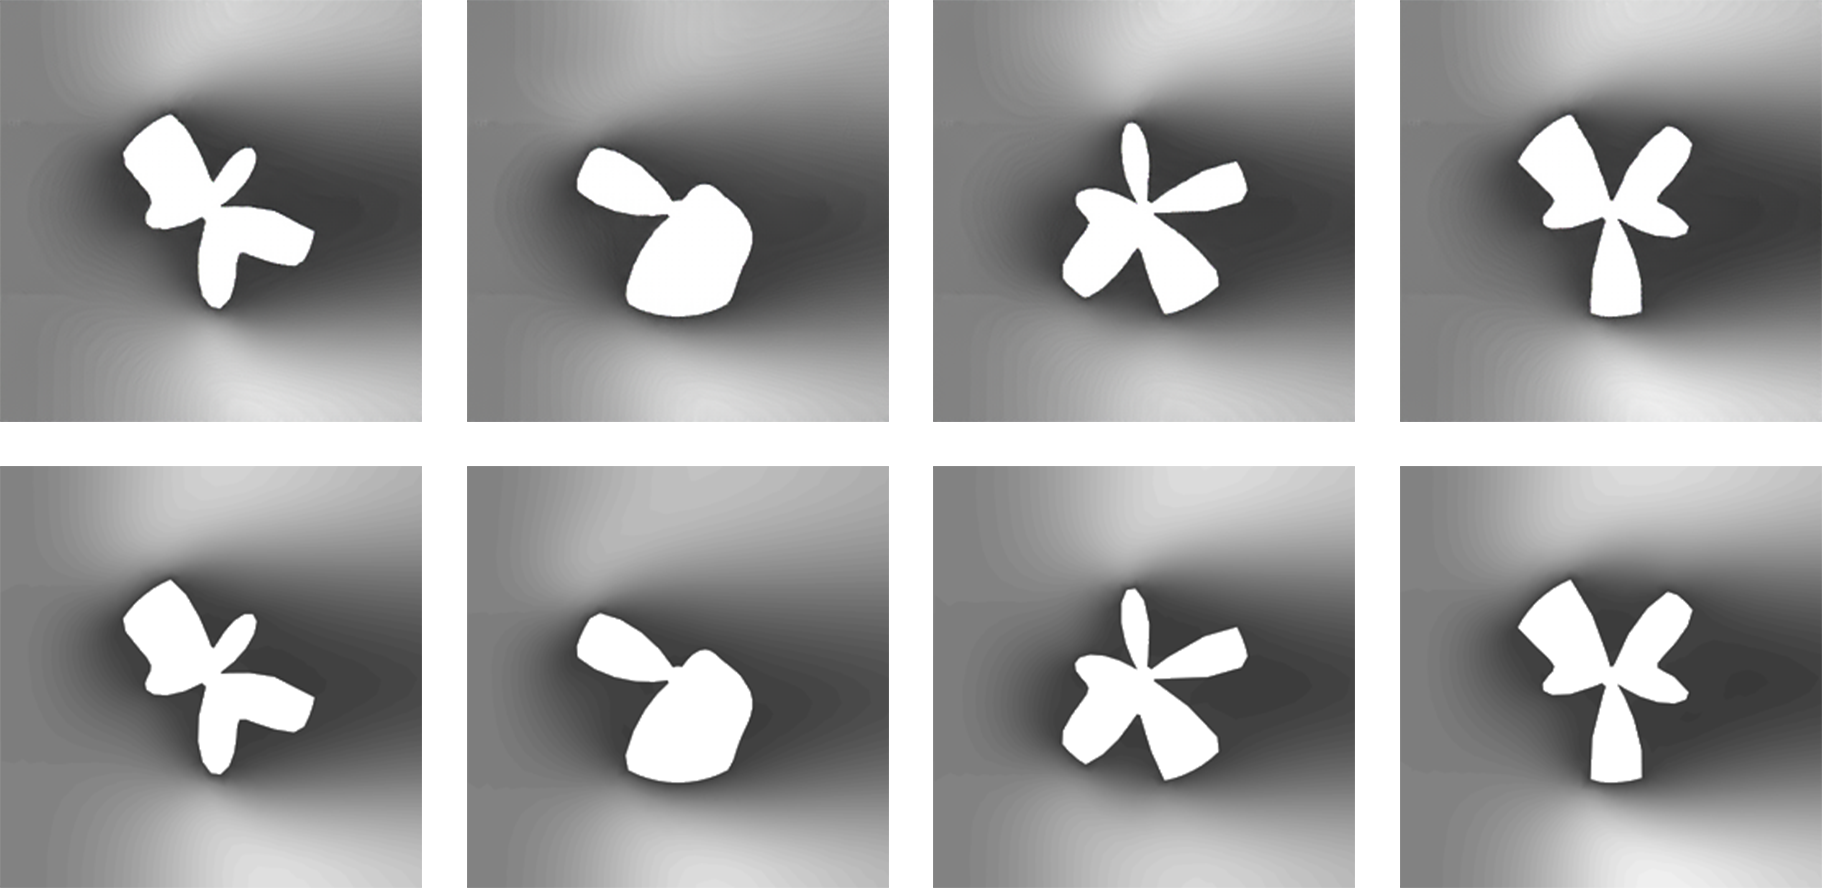
\includegraphics[width=\textwidth]{result2.png}
 \caption{Results on complex shapes. The upper row is neural network's 
prediction. The lower row is the simulated ground truth.}
 \label{fig:result2}
\end{figure}

\begin{figure}[p]
 \centering
 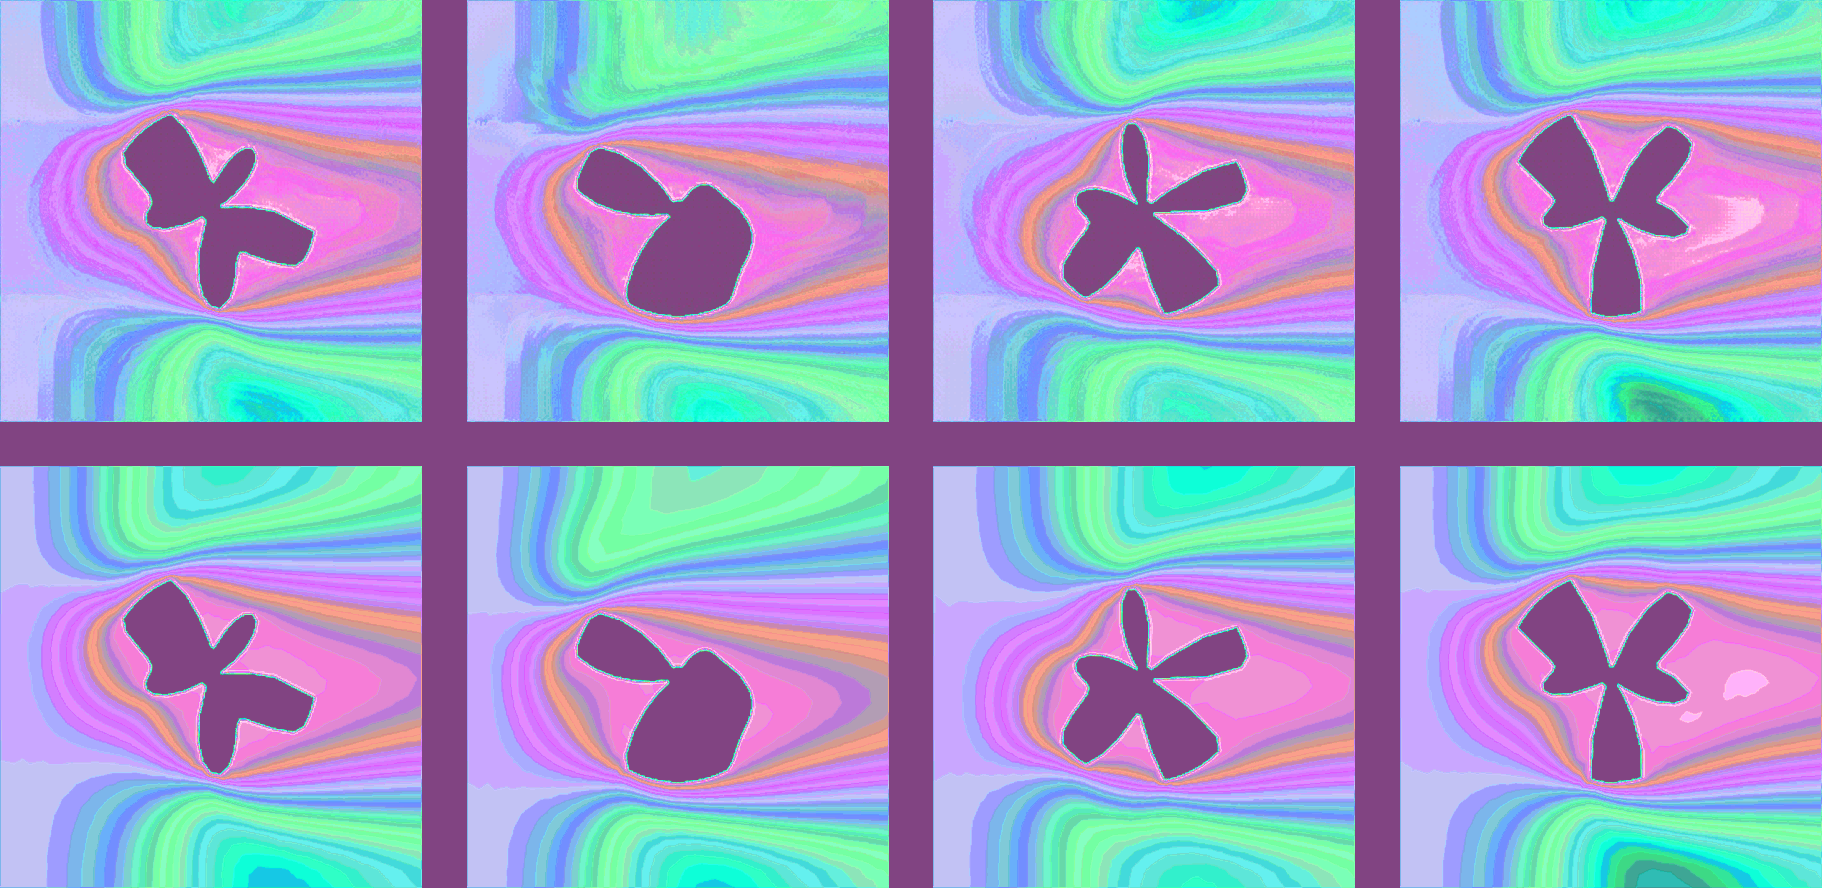
\includegraphics[width=\textwidth]{result2-color.png}
 \caption{Results on complex shapes. Each gray-scale color is randomly 
 replace by another color for better visualization.}
 \label{fig:result2c}
\end{figure}

Figure~\ref{fig:result2} shows the results on complex shapes, and we can see that the prediction is reasonably accurate.
To better analyze the details, we recolor the results in Figure~\ref{fig:result2c}. We find that most of the contour lines are correctly predicted, even when they're asymmetric.
The most obvious error is related with the local optima and closed loop contours, as shown in the rightmost pair of images.
The groundtruth result has two clear circle shapes on the right of the obstacle, but the prediction result blurs them together.

\section{Discussion}

In this project we try to use machine learning models to approximate numerical simulation on 2D fields.
The current approach has strong limitations, such as requiring steady state solutions and lots of training data.
However, we demonstrate the strong capability of use neural network for accurate and fast prediction.
On both simple and complex shapes, the prediction results are reasonably close to the groundtruth results.
With GPU acceleration, the neural networks can achieve about 100$\times$ of speedup comparing to numerical simulation.

For future works, a simple extension is to construct the neural network with 3D-convolution (widely used in video processing) and allow it to process 3D data.
This will greatly extend the range of applications of the current method, and achieve even higher speed up comparing to numerical simulation.

Another interesting direction is to integrate the machine learning approximation with numerical simulation and form a close loop.
In one direction, we can use the approximated solution as an initial value for the numerical solver and then obtain an accurate solution faster.
In the other direction, the machine learning model is continuous learned when the numerical simulator accumulates more data.
As such, accurate result can be guaranteed and no explicit training phase is required.

\bibliographystyle{unsrt}
\bibliography{reference}

\end{document}
